\documentclass[12pt,a4paper]{article}

% Including essential packages for Chinese typesetting
\usepackage{xeCJK}
\usepackage{fontspec}
% Configuring Chinese font with Noto Serif CJK TC, fallback to SimSun
\IfFontExistsTF{Noto Serif CJK TC}{
  \setCJKmainfont{Noto Serif CJK TC}
  \setCJKsansfont{Noto Serif CJK TC}
  \setCJKmonofont{Noto Serif CJK TC}
}{\setCJKmainfont{SimSun}
  \setCJKsansfont{SimSun}
  \setCJKmonofont{SimSun}
}

% Including other necessary packages
\usepackage{geometry}
\usepackage{titlesec}
\usepackage{enumitem}
\usepackage{xcolor}
\usepackage{colortbl}
\usepackage{tcolorbox}
\usepackage{booktabs}
\usepackage{longtable}
\usepackage{array}
\usepackage{graphicx}
\usepackage{tikz}
\usepackage{fancyhdr}
\usepackage{multicol}
\usepackage{datetime2}
\usepackage{hyperref}
\usepackage{mdframed}
\usepackage{amsmath}

\hypersetup{
    colorlinks=true,
    linkcolor=emergency_blue,
    citecolor=emergency_blue,
    urlcolor=emergency_blue,
    pdfborder={0 0 0}
}

% Defining page geometry
\geometry{
  top=2.5cm,
  bottom=2.5cm,
  left=2cm,
  right=2cm,
  headheight=25pt
}

% Adjusting topmargin to compensate for increased headheight
\addtolength{\topmargin}{-10pt}

% Defining colors
\definecolor{emergency_red}{RGB}{186,24,27}
\definecolor{emergency_blue}{RGB}{0,114,188}
\definecolor{emergency_gray}{RGB}{120,120,120}
\definecolor{highlight_yellow}{RGB}{255,250,205}

% Setting title formats
\titleformat{\section}[block]{\Large\bfseries\color{emergency_red}}{\thesection}{10pt}{}
\titleformat{\subsection}[block]{\large\bfseries\color{emergency_blue}}{\thesubsection}{8pt}{}
\titleformat{\subsubsection}[block]{\normalsize\bfseries\color{emergency_gray}}{\thesubsubsection}{6pt}{}

% Defining custom environment for important notes
\newmdenv[
    linecolor=emergency_red,
    backgroundcolor=highlight_yellow,
    linewidth=2pt,
    topline=true,
    bottomline=true,
    leftline=true,
    rightline=true,
    innertopmargin=10pt,
    innerbottommargin=10pt,
    innerleftmargin=10pt,
    innerrightmargin=10pt
]{importantbox}

% Defining note command with tcolorbox
\newcommand{\note}[1]{
    \par
    \noindent
    \begin{tcolorbox}[
        colback=emergency_blue!5!white,
        colframe=emergency_blue,
        title=\textbf{重點提醒},
        fonttitle=\bfseries,
        boxrule=0.5pt,
        arc=3pt,
        left=6pt,
        right=6pt,
        top=6pt,
        bottom=6pt
    ]
    #1
    \end{tcolorbox}
}

% Setting up header and footer
\pagestyle{fancy}
\fancyhf{}
\fancyhead[L]{\textcolor{emergency_red}{USMLE Step 2 CS}}
\fancyhead[R]{\textcolor{emergency_blue}{病史採集與考試技巧}}
\fancyfoot[C]{\textcolor{emergency_gray}{\thepage}}
\renewcommand{\headrulewidth}{1pt}
\renewcommand{\headrule}{\hbox to\headwidth{\color{emergency_red}\leaders\hrule height \headrulewidth\hfill}}

% Defining custom date format for ISO 8601
\DTMnewdatestyle{iso}{
  \renewcommand{\DTMdisplaydate}[4]{\number##1-\number##2-\number##3}
  \renewcommand{\DTMDisplaydate}[4]{\number##1-\number##2-\number##3}
}
\DTMsetdatestyle{iso}
\newcommand{\mydate}{\DTMtoday}

\begin{document}

\begin{titlepage}
    \centering
    \vspace*{2cm}
    {\Huge\bfseries\color{emergency_red} USMLE Step 2 CS\par}
    \vspace{1cm}
    {\LARGE\bfseries 病史收集與考試技巧指引\par}
    \vspace{2cm}
    {\Large Clinical Skills Examination Guide\par}
    \begin{figure}[ht]
        \centering
        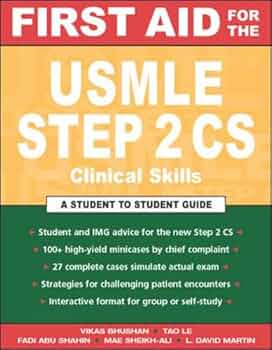
\includegraphics[width=0.5\linewidth]{figure/fig USMLE step 2 CS.png}
    \end{figure}
    \vspace{3cm}
    {\large 編製日期：\mydate\par}
    \vfill
    {\large 適用對象：醫學生、住院醫師\par}
    {\large 編寫: 謝慕揚 MD, PhD, FESC, with assistance by AI: Claude\par}
\end{titlepage}

\tableofcontents
\newpage

\section{考試概述}

\subsection{考試結構}

USMLE Step 2 CS 是一個標準化的臨床技能考試，評估考生與病人互動、病史採集、理學檢查及臨床推理的能力。其中每一站都只有15分鐘完成全部的病史詢問，理學檢查，與手寫記錄。請注意:以上三項是全部在15分鐘內完成。所以強調學生能在有限時間內完成任務，在完整性與時效上均需要兼顧。所以每個學生都需要花心思練習，才能在時間限制內完成任務。

我個人是在2009年自己訓練，在R2期間，用自己的假期去Los Angeles, California, USA完成了第一次考試，第一次考試沒通過，因為我太輕忽，以為好好講完就會通過，結果在English proficiency被勾選: fail. 後來準備了半年，於R3休假期間，再飛去Atlanta, USA完成第二次嘗試，然後才通過。

一個clinical skill考試考了兩次，我可以說我有累積相當的經驗。這個臨床考試很紮實，我學習很多，也讓我在擔任總醫師與主治醫師時，能夠更有自信的完成溝通，並好好的照護病患。

我在2010-2011年編寫了考試心得，之後用這份教材在14CD病房訓練clerks and interns (history taking only), 他們的表情我到現在都忘不了:怎麼三十分鐘可以讓我們這麼有收獲?

後來到了新竹分院擔任心臟內科醫師，也開始忙了，一直到2025年，開始用AI: Claude, 先寫python將過去的筆記與PDF檔案進行文字辨識，再用latex重新編寫全部的資料，完成了這份更新版的教學文件。希望對於同仁們的教學歷程有幫助。



\begin{importantbox}
\textbf{考試時間分配（每個病例15分鐘）：}
\begin{itemize}
    \item 門口資訊閱讀：10-20秒
    \item 病史詢問：7-8分鐘
    \item 理學檢查：3-5分鐘
    \item 關門（Closure）：2-3分鐘
    \item 病歷書寫：10分鐘
\end{itemize}
\end{importantbox}

\subsection{評分標準}

考試評估三個主要面向：
\begin{enumerate}
    \item \textbf{溝通與人際技巧（Communication and Interpersonal Skills, CIS）}
    \item \textbf{整合性臨床會診（Integrated Clinical Encounter, ICE）}
    \item \textbf{口語能力（Spoken English Proficiency, SEP）}
\end{enumerate}

\section{時間管理策略}

\note{時間管理是通過考試的關鍵。考生必須在15分鐘內完成所有任務，任何時間的浪費都可能導致無法完成必要的步驟。}

\subsection{常見時間不足的原因}

\begin{enumerate}
    \item 詢問過於詳細的病史
    \item 進行不必要的詳細理學檢查
    \item 以緩慢或無組織的方式進行會診
    \item 允許病人離題討論不相關的話題
    \item 無法適當控制具有挑戰性的病人（如：不合作、憤怒、過度焦慮）
\end{enumerate}

\subsection{時間管理技巧}

\begin{itemize}
    \item 使用「五分鐘提醒」作為唯一的時間指標
    \item 聽到五分鐘提醒時，應該已經開始理學檢查
    \item 將手錶轉半圈戴在手腕上，可以在不明顯看錶的情況下掌握時間
    \item 有組織且計劃良好的病史詢問是關鍵
    \item 進行簡短而聚焦的理學檢查
    \item 不要為了節省時間而忽略病人的問題、請求或情緒狀態
\end{itemize}

\section{病史採集技巧}

\subsection{開場與建立關係}

\subsubsection{入門檢查清單}

\begin{tcolorbox}[colback=emergency_blue!10!white,colframe=emergency_blue,title=入場標準流程]
\begin{enumerate}
    \item 敲門後進入
    \item 自我介紹（姓名）
    \item 說明自己的角色或職位
    \item 正確使用病人姓名
    \item 與標準化病人保持眼神接觸
\end{enumerate}
\end{tcolorbox}

\subsubsection{開場用語範例}

\begin{itemize}
    \item "Good morning, Mr. Jones. I am Dr. Singh. It's nice to meet you."
    \item "How can I help you today?"
    \item "What brought you to the hospital/clinic today?"
\end{itemize}

\subsection{病史詢問架構：FOPQRST}

\note{使用 FOPQRST 記憶法系統化地詢問症狀，確保不遺漏重要資訊。}

\begin{longtable}{>{\bfseries}p{3cm}p{10cm}}
\toprule
\textbf{項目} & \textbf{詢問內容} \\
\midrule
\endhead
F - Frequency & 頻率：多久發生一次？\\
\midrule
O - Onset & 發作：什麼時候開始的？如何開始的？\\
\midrule
P - Precipitating \newline factors & 誘發因素：什麼情況下會發生？有什麼會引發？\\
\midrule
Q - Quality & 性質：是什麼樣的感覺？（尖銳、鈍痛、灼熱、壓迫感等）\\
\midrule
R - Radiation & 放射：疼痛會擴散到其他地方嗎？\\
\midrule
S - Severity & 嚴重程度：1-10分，10分是最嚴重，你會給幾分？\\
\midrule
T - Timing & 時間：持續多久？是持續性還是間歇性？\\
\bottomrule
\end{longtable}

\subsection{完整病史架構}

\begin{enumerate}
    \item \textbf{主訴（Chief Complaint）}
    \item \textbf{現病史（History of Present Illness, HPI）}
    \begin{itemize}
        \item 使用 FOPQRST 詢問主要症狀
        \item 相關症狀（Associated symptoms）
        \item 緩解/惡化因素（Alleviating/Exacerbating factors）
        \item 過去類似發作（Previous episodes）
    \end{itemize}
    \item \textbf{系統回顧（Review of Systems, ROS）}
    \item \textbf{過去病史（Past Medical History, PMH）}
    \item \textbf{過去手術史（Past Surgical History, PSH）}
    \item \textbf{用藥史（Medications）}
    \item \textbf{過敏史（Allergies）}
    \item \textbf{家族史（Family History, FH）}
    \item \textbf{社會史（Social History, SH）}
    \begin{itemize}
        \item 職業
        \item 居住狀況
        \item 吸菸史（CAGE評估）
        \item 飲酒史（量、頻率）
        \item 藥物使用史
        \item 性生活史（如適用）
    \end{itemize}
\end{enumerate}

\subsection{常見症狀詢問要點}

\subsubsection{疼痛（Pain）}

\begin{itemize}
    \item "Do you have pain?"
    \item "When did it start?"
    \item "Where do you feel the pain? Can you show me exactly where it is?"
    \item "Does the pain travel anywhere?"
    \item "What is the pain like? Can you describe it for me?"
    \item "On a scale of 1 to 10, with 10 being the worst pain of your life, how would you rate your pain?"
    \item "What brings the pain on?"
    \item "Does anything make the pain better or worse?"
\end{itemize}

\subsubsection{呼吸困難（Shortness of Breath）}

\begin{itemize}
    \item "Do you get short of breath?"
    \item "When did it start?"
    \item "Does it happen when you climb stairs? How many steps can you climb before you get short of breath?"
    \item "What makes it worse? What makes it better?"
    \item "Do you wake up at night short of breath?"
    \item "Do you have to prop yourself up on pillows to sleep? How many?"
    \item "Have you been wheezing?"
\end{itemize}

\subsubsection{頭痛（Headache）}

\begin{itemize}
    \item "Tell me about your headaches."
    \item "When do your headaches start? How often do you get them?"
    \item "Can you show me exactly where you feel the headache?"
    \item "What causes the headache to start?"
    \item "What makes it worse? What makes it better?"
    \item "Can you describe the headache? Is it sharp, dull, pulsating, or pressure-like?"
    \item "Do you notice any change in your vision before/during/after the headaches?"
    \item "Do you feel nauseated? Do you vomit?"
\end{itemize}

\section{理學檢查}

\subsection{檢查前準備}

\begin{importantbox}
\textbf{檢查前必做事項：}
\begin{enumerate}
    \item 洗手（使用肥皂和水，或酒精性乾洗手液）
    \item 告知病人你將要進行的檢查
    \item 請求病人同意解開病袍
    \item 適當地使用布簾遮蔽病人
\end{enumerate}
\end{importantbox}

\subsection{檢查原則}

\note{理學檢查應該聚焦且有組織。不要試圖進行全面性的理學檢查，而是針對鑑別診斷進行相關系統的檢查。}

\begin{enumerate}
    \item 保持檢查聚焦且有組織
    \item 盡可能少暴露病人身體
    \item 不要隔著病袍進行檢查
    \item 從遠離疼痛區域開始檢查
    \item 不要重複引起疼痛的操作
    \item 檢查完畢後立即覆蓋病人
    \item 每個步驟都要說明並徵得同意
\end{enumerate}

\subsection{禁止的檢查項目}

\begin{tcolorbox}[colback=emergency_red!10!white,colframe=emergency_red,title=\textbf{禁止進行的檢查}]
考試中\textbf{不允許}進行以下檢查：
\begin{itemize}
    \item 角膜反射（Corneal reflex）
    \item 乳房檢查（Breast exam）
    \item 直腸檢查（Rectal exam）
    \item 骨盆檢查（Pelvic exam）
    \item 生殖器檢查（Genital exam）
\end{itemize}

如果認為需要進行上述檢查，應該：
\begin{enumerate}
    \item 告知病人稍後需要進行該檢查
    \item 在病歷的診斷計畫中註明該檢查項目
\end{enumerate}
\end{tcolorbox}

\subsection{系統性理學檢查}

\subsubsection{HEENT 檢查}

\textbf{檢查前說明：}
\begin{itemize}
    \item "I need to examine your sinuses, so I am going to press on your forehead and cheeks."
    \item "I would like to examine your eyes now. I am going to shine this light in your eyes."
    \item "Can you please open your mouth? I need to check the inside of your mouth and your throat."
\end{itemize}

\textbf{檢查項目：}
\begin{itemize}
    \item \textbf{頭部：}檢查外傷跡象、疤痕；觸診壓痛或異常
    \item \textbf{眼睛：}鞏膜和結膜；瞳孔對光反應；眼球運動；視力（使用 Snellen 視力表）
    \item \textbf{耳朵：}外耳檢查；耳道和鼓膜（使用耳鏡）；Rinne 和 Weber 測試
    \item \textbf{鼻子：}檢查鼻腔；觸診鼻子和鼻竇
    \item \textbf{口腔和喉嚨：}使用光源檢查
\end{itemize}

\subsubsection{心血管檢查}

\textbf{檢查前說明：}
\begin{itemize}
    \item "I need to listen to your heart."
    \item "Can you hold your breath, please?"
    \item "Can you sit up, please?"
    \item "Can you turn to your left side, please?"
\end{itemize}

\textbf{檢查項目：}
\begin{itemize}
    \item 頸動脈聽診（檢查雜音）
    \item 檢查頸靜脈怒張（JVD）
    \item 觸診胸部（PMI、retrosternal heave、thrills）
    \item 聽診至少兩個心臟區域
    \item 檢查下肢水腫
    \item 檢查周邊脈搏
\end{itemize}

\subsubsection{肺部檢查}

\textbf{檢查前說明：}
\begin{itemize}
    \item "I need to listen to your lungs now."
    \item "Can you take a deep breath for me, please?"
    \item "Can you say '99' for me, please?"
    \item "I am going to tap on your back to check your lungs."
\end{itemize}

\textbf{檢查項目：}
\begin{itemize}
    \item 檢查胸部前後
    \item 視診：胸部形狀、呼吸型態、變形
    \item 觸診：壓痛、tactile fremitus
    \item 叩診
    \item 聽診、egophony
\end{itemize}

\subsubsection{腹部檢查}

\textbf{檢查前說明：}
\begin{itemize}
    \item "I need to examine your belly/stomach now."
    \item "I am going to listen to your belly now."
    \item "I am going to press on your belly. Tell me if you feel any pain or discomfort."
    \item "Do you feel any pain when I press in or when I let go?"
\end{itemize}

\textbf{檢查項目（按順序）：}
\begin{enumerate}
    \item 視診
    \item 聽診（\textbf{在觸診前進行}）
    \item 叩診
    \item 觸診：從遠離疼痛點開始；檢查反彈壓痛、CVA 壓痛、Murphy's sign
    \item 檢查肝臟範圍
\end{enumerate}

\section{關門技巧（Closure）}

\subsection{關門的目的}

\note{關門是病人會談的關鍵部分，用於：(1) 總結發現；(2) 解釋初步印象；(3) 說明診斷計畫；(4) 回答病人問題；(5) 處理病人關切。}

\subsection{關門步驟}

\begin{enumerate}
    \item \textbf{轉換語句}
    \begin{itemize}
        \item "Thank you for letting me examine you, Mrs. Jones. Now I would like to sit down with you and give you my impression."
    \end{itemize}
    
    \item \textbf{簡要總結}
    \begin{itemize}
        \item 總結主訴和重要病史（如之前未做）
        \item 總結理學檢查發現
    \end{itemize}
    
    \item \textbf{說明初步印象}
    \begin{itemize}
        \item 提出可能的鑑別診斷（最多3個）
        \item 使用簡單的非醫學術語解釋
        \item \textbf{不要}給出確定診斷
    \end{itemize}
    
    \item \textbf{說明診斷計畫}
    \begin{itemize}
        \item 解釋計劃進行的檢查
        \item 使用非技術性語言
        \item 例如："We need to run some blood tests to check the function of your liver and kidney."
    \end{itemize}
    
    \item \textbf{回答問題並處理關切}
    \begin{itemize}
        \item 誠實但圓融
        \item 避免給予虛假的保證
        \item 如果不知道答案，坦白告知
    \end{itemize}
    
    \item \textbf{告別}
    \begin{itemize}
        \item "I will contact you when I have your test results."
        \item "It was nice meeting you."
        \item 與病人握手
    \end{itemize}
\end{enumerate}

\subsection{處理挑戰性問題}

\subsubsection{關於診斷的問題}

\begin{tcolorbox}[colback=highlight_yellow,colframe=emergency_gray]
\textbf{病人：}"Is this a heart attack? Am I going to die?"

\textbf{回應範例：}"Given your current presentation, my suspicion for a heart attack is low. It is more likely that inflammation of the membranes surrounding your lungs is causing your pain, and this is usually not a life-threatening condition. However, we still need to do some tests to confirm the diagnosis and rule out heart problems."
\end{tcolorbox}

\subsubsection{關於癌症的問題}

\begin{tcolorbox}[colback=highlight_yellow,colframe=emergency_gray]
\textbf{病人：}"Do you think I have cancer?"

\textbf{回應範例：}"That is one of the possibilities, but there are other explanations for your symptoms that we should rule out before making a diagnosis."
\end{tcolorbox}

\subsubsection{關於預後的問題}

\begin{tcolorbox}[colback=highlight_yellow,colframe=emergency_gray]
\textbf{病人：}"Will I ever feel better, doctor?"

\textbf{回應範例：}根據疾病預後不同，可以從"Yes, most people with this disease are completely cured"到"Complete cure may be difficult at this advanced stage, but we have a lot to offer in terms of controlling the symptoms and improving your quality of life."
\end{tcolorbox}

\section{病歷書寫（Patient Note）}

\subsection{病歷結構}

病歷包含四個主要部分：

\begin{enumerate}
    \item \textbf{病史（History）}
    \item \textbf{理學檢查（Physical Examination）}
    \item \textbf{鑑別診斷（Differential Diagnosis）}
    \item \textbf{初步診斷計畫（Initial Diagnostic Workup）}
\end{enumerate}

\subsection{病史書寫要點}

\note{病史應該清晰、直接、簡潔。避免冗長複雜的句子。使用標準醫學縮寫以節省空間和時間。}

\textbf{必須包含的內容：}
\begin{itemize}
    \item 主訴（CC）
    \item 現病史（HPI）
    \item 系統回顧（ROS）
    \item 過去病史（PMH）
    \item 過去手術史（PSH）
    \item 社會史（SH）
    \item 家族史（FH）
\end{itemize}

\subsection{理學檢查記錄範例}

\begin{tcolorbox}[colback=emergency_blue!5!white,colframe=emergency_blue]
\textbf{Patient is in severe pain.}

\textbf{VS:} BP 165/85 (both arms), RR 22

\textbf{Neck:} No JVD, no bruits

\textbf{Chest:} No tenderness, clear symmetric breath sounds bilaterally

\textbf{Heart:} Apical impulse not displaced; RRR; normal S1/S2; no murmurs, rubs, or gallops

\textbf{Abdomen:} Soft, nondistended, nontender; +BS; no hepatosplenomegaly

\textbf{Extremities:} No edema, peripheral pulses 2+ and symmetric
\end{tcolorbox}

\subsection{鑑別診斷與診斷計畫}

\begin{importantbox}
\textbf{重要原則：}
\begin{itemize}
    \item 鑑別診斷：最多列出5個，從最可能到最不可能排列
    \item 診斷計畫：最多列出5項檢查
    \item 從簡單到複雜排列檢查
    \item 如需要，先列出「禁止的理學檢查」（直腸檢查、骨盆檢查等）
    \item 要具體：不要寫"chem 7"，要寫"Na, K, Cl, CO2, BUN, Cr, glucose"
    \item \textbf{不要}包括會診、治療、住院或轉診
\end{itemize}
\end{importantbox}

\section{標準案例：急性胸痛}

\subsection{案例資訊}

\begin{tcolorbox}[colback=emergency_red!10!white,colframe=emergency_red,title=\textbf{門口資訊（Doorway Information）}]
\textbf{Opening Scenario:} Joseph Short, a 46-year-old male, comes to the ER complaining of chest pain.

\textbf{Vital Signs:}
\begin{itemize}
    \item BP: 165/85 mmHg
    \item Temp: 98.6°F (37°C)
    \item RR: 22/minute
    \item HR: 91/minute, regular
\end{itemize}

\textbf{Examinee Tasks:}
\begin{enumerate}
    \item Take a focused history
    \item Perform a focused physical exam (do not perform rectal, genitourinary, or female breast exams)
    \item Explain your clinical impression and workup plan to the patient
    \item Write the patient note after leaving the room
\end{enumerate}
\end{tcolorbox}

\subsection{標準化病人回應}

\begin{longtable}{>{\bfseries}p{5cm}p{9cm}}
\toprule
\textbf{問題} & \textbf{標準化病人回應} \\
\midrule
\endhead
Chief complaint & Chest pain. \\
\midrule
Onset & Forty minutes ago. \\
\midrule
Precipitating events & Nothing; I was asleep and I woke up at 5:00 in the morning having this pain. \\
\midrule
Progression & Constant \\
\midrule
Severity & 7/10 \\
\midrule
Location & Middle of the chest. \\
\midrule
Radiation & To my neck and left arm. \\
\midrule
Quality & Pressure \\
\midrule
Alleviating/exacerbating factors & Nothing \\
\midrule
Shortness of breath & Yes. \\
\midrule
Nausea/vomiting & I feel nauseated, but I didn't vomit. \\
\midrule
Sweating & Yes. \\
\midrule
Associated symptoms & None mentioned \\
\midrule
Previous episodes & Yes, but not exactly the same. \\
\midrule
Onset of previous episodes & Past three months \\
\midrule
Severity of previous episodes & Less severe \\
\midrule
Frequency & Two to three episodes a week \\
\midrule
Precipitating factors & Walking up the stairs, strenuous work, and heavy meals \\
\midrule
Alleviating factors & Antacids \\
\midrule
Associated symptoms & None \\
\midrule
Current medications & Maalox, diuretic \\
\midrule
Past medical history & Hypertension for five years, treated with a diuretic. High cholesterol, managed with diet; have not been very compliant with the diet. GERD 10 years ago, treated with antacids. \\
\midrule
Past surgical history & None \\
\midrule
Family history & My father died of lung cancer. My mother is alive and has a peptic ulcer. No early heart attacks. \\
\midrule
Occupation & Accountant \\
\midrule
Alcohol use & Once in a while \\
\midrule
Illicit drug use & Cocaine, once a week \\
\midrule
Last time of cocaine use & Yesterday afternoon \\
\midrule
Tobacco & One pack a day for 25 years; stopped three months ago \\
\midrule
Sexual activity & "I haven't had sex with my wife for the last three months because, to be honest, I get this pain in my chest during sex." \\
\midrule
Exercise & No \\
\midrule
Diet & "My doctor gave me a strict diet last year to lower my cholesterol, but I always cheat." \\
\midrule
Drug allergies & No \\
\bottomrule
\end{longtable}

\subsection{標準關門回應範例}

\begin{tcolorbox}[colback=highlight_yellow,colframe=emergency_blue,title=\textbf{Sample Closure}]
"Mr. Short, the source of your pain can be a cardiac problem such as a heart attack or angina, or it may be due to acid reflux, lung problems, or disorders related to the large blood vessels in your chest. It is crucial that we perform some tests in order to identify the source of your problem. We will start with an ECG and some blood work, but more complex tests may be needed as well. In the meantime, we would strongly recommend that you stop using cocaine, since use of this drug can lead to a variety of medical problems, including heart attacks. Do you have any questions for me?"
\end{tcolorbox}

\subsection{理學檢查檢查清單}

\begin{tcolorbox}[colback=emergency_gray!10!white,colframe=emergency_gray]
\textbf{應進行的檢查：}
\begin{itemize}
    \item Neck exam: Look for JVD, carotid auscultation
    \item CV exam: Inspection, palpation, auscultation
    \item Pulmonary exam: Auscultation, palpation, percussion
    \item Abdominal exam: Auscultation, palpation, percussion
    \item Extremities: Check peripheral pulses, check blood pressure in both arms, look for edema
\end{itemize}
\end{tcolorbox}

\subsection{鑑別診斷}

\begin{enumerate}
    \item \textbf{心肌缺血或梗塞（Myocardial ischemia or infarction）}
    
    病人有多項心臟危險因子（吸菸、高血壓、高血脂），症狀典型。
    
    \item \textbf{可卡因誘發的心肌缺血（Cocaine-induced myocardial ischemia）}
    
    可卡因可透過冠狀動脈痙攣、增加心肌能量需求或加速動脈粥樣硬化來誘發心肌缺血和梗塞。
    
    \item \textbf{胃食道逆流（GERD）}
    
    嚴重胸痛是 GERD 的非典型但常見症狀，可能在夜間平躺時惡化。
    
    \item \textbf{主動脈剝離（Aortic dissection）}
    
    雖然病人的疼痛不是典型的撕裂性胸痛放射到背部，但因其突然發作的嚴重胸痛和死亡風險，仍需考慮。
    
    \item \textbf{心包炎（Pericarditis）}
    
    沒有隨姿勢或呼吸改變的疼痛，也沒有心包摩擦音，較不可能。
    
    \item \textbf{氣胸（Pneumothorax）}
    
    急性胸痛和呼吸困難應考慮，但雙側呼吸音對稱使其較不可能。
    
    \item \textbf{肺栓塞（Pulmonary embolism）}
    
    急性胸痛和呼吸困難的鑑別診斷之一，但此病人沒有明顯的危險因子。
    
    \item \textbf{肋軟骨炎（Costochondritis）}
    
    典型與觸診疼痛或胸膜性疼痛相關。
\end{enumerate}

\subsection{診斷計畫}

\begin{enumerate}
    \item \textbf{心電圖（ECG）}
    
    急性心肌缺血、梗塞和心包炎在心電圖上有特徵性變化。
    
    \item \textbf{心臟酵素（Cardiac enzymes: CPK, CPK-MB, troponin）}
    
    檢測心肌組織壞死的特異性測試，疼痛發作後4-6小時可能轉為陽性。
    
    \item \textbf{胸部X光（CXR）}
    
    縱膈增寬提示主動脈剝離，也可診斷其他胸痛原因，包括氣胸和肺炎。
    
    \item \textbf{經胸超音波心臟圖（Transthoracic echocardiogram, TTE）}
    
    可顯示急性心肌梗塞的節段性壁運動異常。
    
    \item \textbf{心導管檢查（Cardiac catheterization）}
    
    可診斷和治療冠狀動脈疾病。
    
    \item \textbf{經食道超音波心臟圖（Transesophageal echocardiogram, TEE）}
    
    對主動脈剝離高度特異和敏感，可在床邊快速完成。
    
    \item \textbf{胸部電腦斷層（CT chest with IV contrast）}
    
    另一個可快速排除主動脈剝離或肺栓塞的診斷工具。
    
    \item \textbf{上消化道內視鏡（Upper endoscopy）}
    
    可記錄 GERD 特徵性的組織損傷。
    
    \item \textbf{膽固醇檢測（Cholesterol panel）}
    
    可識別心血管疾病的關鍵危險因子。
\end{enumerate}

\section{特殊情況處理}

\subsection{處理焦慮的病人}

\begin{itemize}
    \item 鼓勵病人談論感受
    \item 詢問造成焦慮的原因
    \item 給予合理的保證
\end{itemize}

\subsection{處理憤怒的病人}

\begin{itemize}
    \item 保持冷靜，不要害怕
    %\item 記住病人只是在演戲測試你的反應
    \item 讓病人表達感受
    \item 詢問憤怒的原因
    \item 以合理的方式處理病人的憤怒
\end{itemize}

\textbf{範例：}
\begin{quote}
病人："Where have you been, doctor? I have been waiting here for the whole day."

回應："I am sorry you had to wait so long. We had some unexpected delays with a few of the earlier patients this morning. But I'm here now, and I will focus on you and your concerns."
\end{quote}

\subsection{處理哭泣的病人}

\begin{itemize}
    \item 允許病人表達感受
    \item 安靜等待病人完成
    \item 遞送面紙
    \item 在臉部表情中展現同理心
    \item 可以輕輕將手放在病人肩膀或手臂上
    \item 說："I know that you feel sad. Would you like to tell me about it?"
\end{itemize}

\subsection{處理疼痛的病人}

\begin{itemize}
    \item 表現對病人疼痛的同情
    \item 說："I know that you are in pain."
    \item 提供協助："Is there anything I can do for you to help you feel more comfortable?"
    \item 如果病人因疼痛不允許檢查，解釋檢查的必要性
\end{itemize}

\subsection{處理拒絕回答或檢查的病人}

\begin{itemize}
    \item 解釋為什麼問題或檢查很重要
    \item 告知這對理解問題和做出診斷是必要的
    \item 如果病人仍拒絕合作，跳過該問題或操作
    \item 在病歷中記錄病人的拒絕和你的建議
\end{itemize}

\section{衛教與諮商}

\subsection{戒菸諮商（5A's 架構）}

\begin{enumerate}
    \item \textbf{Ask（詢問）:} 詢問病人的吸菸狀況
    \item \textbf{Advise（建議）:} 建議病人戒菸
    \item \textbf{Assess（評估）:} 評估病人戒菸的意願
    \item \textbf{Assist（協助）:} 協助病人戒菸計畫
    \item \textbf{Arrange（安排）:} 安排後續追蹤
\end{enumerate}

\textbf{對話範例：}

\begin{tcolorbox}[colback=emergency_blue!5!white,colframe=emergency_blue]
\textbf{Examinee:} "Do you smoke cigarettes?"

\textbf{SP:} "Yes, I have smoked one pack a day for 20 years."

\textbf{Examinee:} "Have you ever tried to quit?"

\textbf{SP:} "Of course, but it never works."

\textbf{Examinee:} "Well, I strongly recommend that you quit smoking. Smoking is a major cause of cancer and heart disease. Are you interested in trying to quit now?"

\textbf{SP:} "Yes."

\textbf{Examinee:} "I would be happy to help you quit smoking. We have many tools to help you do that, and I will be with you every step of the way. Let's set up an appointment for two weeks from today, and we can get started on it then. Is that okay with you?"
\end{tcolorbox}

\subsection{酒精使用評估（CAGE 問卷）}

\begin{importantbox}
\textbf{CAGE 問卷：}
\begin{enumerate}
    \item \textbf{C}ut down: Have you ever felt the need to \textbf{cut down} on your drinking?
    \item \textbf{A}nnoyed: Have you ever felt \textbf{annoyed} by criticism of your drinking?
    \item \textbf{G}uilty: Have you ever had \textbf{guilty} feelings about drinking?
    \item \textbf{E}ye opener: Have you ever had a drink first thing in the morning (\textbf{eye opener}) to steady your nerves or get rid of a hangover?
\end{enumerate}

\textbf{任何一個問題回答「是」都應該引起懷疑並進一步詢問。}
\end{importantbox}

\subsection{性行為安全諮商}

\textbf{對話範例：}

\begin{tcolorbox}[colback=emergency_blue!5!white,colframe=emergency_blue]
\textbf{Examinee:} "Are you using any type of protection with these partners?"

\textbf{SP:} "My girlfriend is on the pill, but I don't use anything with the other women I see."

\textbf{Examinee:} "Condoms reduce the risk of sexually transmitted infections. Do you think you could try to use condoms?"

\textbf{SP:} "I tried them, but I just don't like them."

\textbf{Examinee:} "I understand that you may not like to use condoms, but I am concerned that you may be putting yourself at risk for STDs. You could contract HIV, herpes, chlamydia, or any of a number of other STDs. The complications of these diseases include infertility, painful infections, or even death. If anyone with whom you have sexual contact has an STD, you could share it among all of them, including your girlfriend. I hope you will consider using a condom in the future. Do you have any questions for me?"
\end{tcolorbox}

\section{考試準備建議}

\subsection{練習要點}

\begin{enumerate}
    \item \textbf{時間管理練習}
    \begin{itemize}
        \item 使用計時器模擬15分鐘的會談
        \item 練習在10分鐘內完成病歷書寫
        \item 熟悉何時該轉換到下一個階段
    \end{itemize}
    
    \item \textbf{病史詢問練習}
    \begin{itemize}
        \item 記憶並練習 FOPQRST 架構
        \item 熟記常見症狀的詢問要點
        \item 練習流暢的開場白和轉換語句
    \end{itemize}
    
    \item \textbf{理學檢查練習}
    \begin{itemize}
        \item 練習系統性的檢查流程
        \item 熟記檢查前的說明語句
        \item 練習適當的遮蔽和尊重
    \end{itemize}
    
    \item \textbf{關門技巧練習}
    \begin{itemize}
        \item 練習總結病史和發現
        \item 練習用非專業術語解釋診斷
        \item 準備回應常見的挑戰性問題
    \end{itemize}
    
    \item \textbf{病歷書寫練習}
    \begin{itemize}
        \item 練習使用標準醫學縮寫
        \item 練習簡潔清楚的書寫風格
        \item 熟悉病歷格式和空間限制
    \end{itemize}
\end{enumerate}

\subsection{考試當天注意事項}

\begin{importantbox}
\textbf{考試日檢查清單：}
\begin{itemize}
    \item 提早到達考場（至少30分鐘）
    \item 攜帶有效身份證件
    \item 穿著專業舒適的服裝
    \item 準備聽診器（考場通常有提供）
    \item 確認決定手寫或打字病歷（全部病歷必須使用相同方式）
    \item 放鬆心情，保持自信
\end{itemize}
\end{importantbox}

\section{常用醫學縮寫}

\begin{multicols}{2}
\begin{itemize}
    \item BP = Blood Pressure
    \item HR = Heart Rate
    \item RR = Respiratory Rate
    \item Temp = Temperature
    \item VS = Vital Signs
    \item CC = Chief Complaint
    \item HPI = History of Present Illness
    \item PMH = Past Medical History
    \item PSH = Past Surgical History
    \item FH = Family History
    \item SH = Social History
    \item ROS = Review of Systems
    \item NKDA = No Known Drug Allergies
    \item JVD = Jugular Venous Distension
    \item PMI = Point of Maximal Impulse
    \item RRR = Regular Rate and Rhythm
    \item HEENT = Head, Eyes, Ears, Nose, Throat
    \item CV = Cardiovascular
    \item GI = Gastrointestinal
    \item GU = Genitourinary
    \item CNS = Central Nervous System
    \item EOMI = Extraocular Movements Intact
    \item PERRLA = Pupils Equal, Round, Reactive to Light and Accommodation
    \item DTRs = Deep Tendon Reflexes
    \item LAD = Lymphadenopathy
    \item BS = Bowel Sounds
    \item WNL = Within Normal Limits
\end{itemize}
\end{multicols}

\section{總結}

USMLE Step 2 CS 考試評估的是臨床技能的整合應用，包括溝通能力、病史採集、理學檢查、臨床推理和病歷書寫。成功通過考試的關鍵在於：

\begin{enumerate}
    \item \textbf{充分練習：}熟能生巧，反覆練習直到流暢自然
    \item \textbf{時間管理：}嚴格控制每個階段的時間分配
    \item \textbf{系統化方法：}使用 FOPQRST 等記憶法系統化詢問
    \item \textbf{同理心與尊重：}始終展現對病人的關心和尊重
    \item \textbf{誠實溝通：}對不確定的事項保持誠實，避免虛假保證
    \item \textbf{完整記錄：}確保病歷包含所有必要資訊且字跡清晰
\end{enumerate}

\vspace{1cm}

\begin{center}
\textcolor{emergency_red}{\Large\textbf{祝各位同學學習順利！}}
\end{center}

\end{document}